%%%%%%%%%%%%%%%%%%%%%%%%%%%%%%%%%%%%%%%%%%%%%%%%%%%%%%%%%%%%%%%%%%%%%%%%%%%%%%%%
% experiment.tex: Chapter describing the experiment
%%%%%%%%%%%%%%%%%%%%%%%%%%%%%%%%%%%%%%%%%%%%%%%%%%%%%%%%%%%%%%%%%%%%%%%%%%%%%%%%
\chapter{The NOvA Experiment}
\label{experiment_chapter}
%%%%%%%%%%%%%%%%%%%%%%%%%%%%%%%%%%%%%%%%%%%%%%%%%%%%%%%%%%%%%%%%%%%%%%%%%%%%%%%%

The neutrinos studied by NOvA begin at Fermi National Accelerator Laboratory (Fermilab) 
in Illinois.  An intense muon (anti-)neutrino beam is created at Fermilab by the Neutrino 
at the Main Injector (NuMI) source. NOvA, which stands for NuMI Off-Axis $\nu_e$ Appearance, 
is a long baseline experiment which is designed to determine the neutrino mass hierarchy, 
the octant of $\theta_{23}$, and to measure the CP violating phase $\delta_{CP}$ by measuring 
electron (anti-)neutrino appearance probability and muon (anti-)neutrino disappearance. It 
consists of the Near Detector (ND), which is located at Fermilab and measures total flux of 
neutrino, and the Far Detector (FD), which is located near Ash River, Minnesota and measures 
flux of muon and electron neutrinos. The structures of the NuMI source and the Near and 
Far Detectors, and the detector positions relative to the beam axis will be explained in 
the following sections.

\section{NuMI and Off-Axis Detectors Position}
\begin{figure}
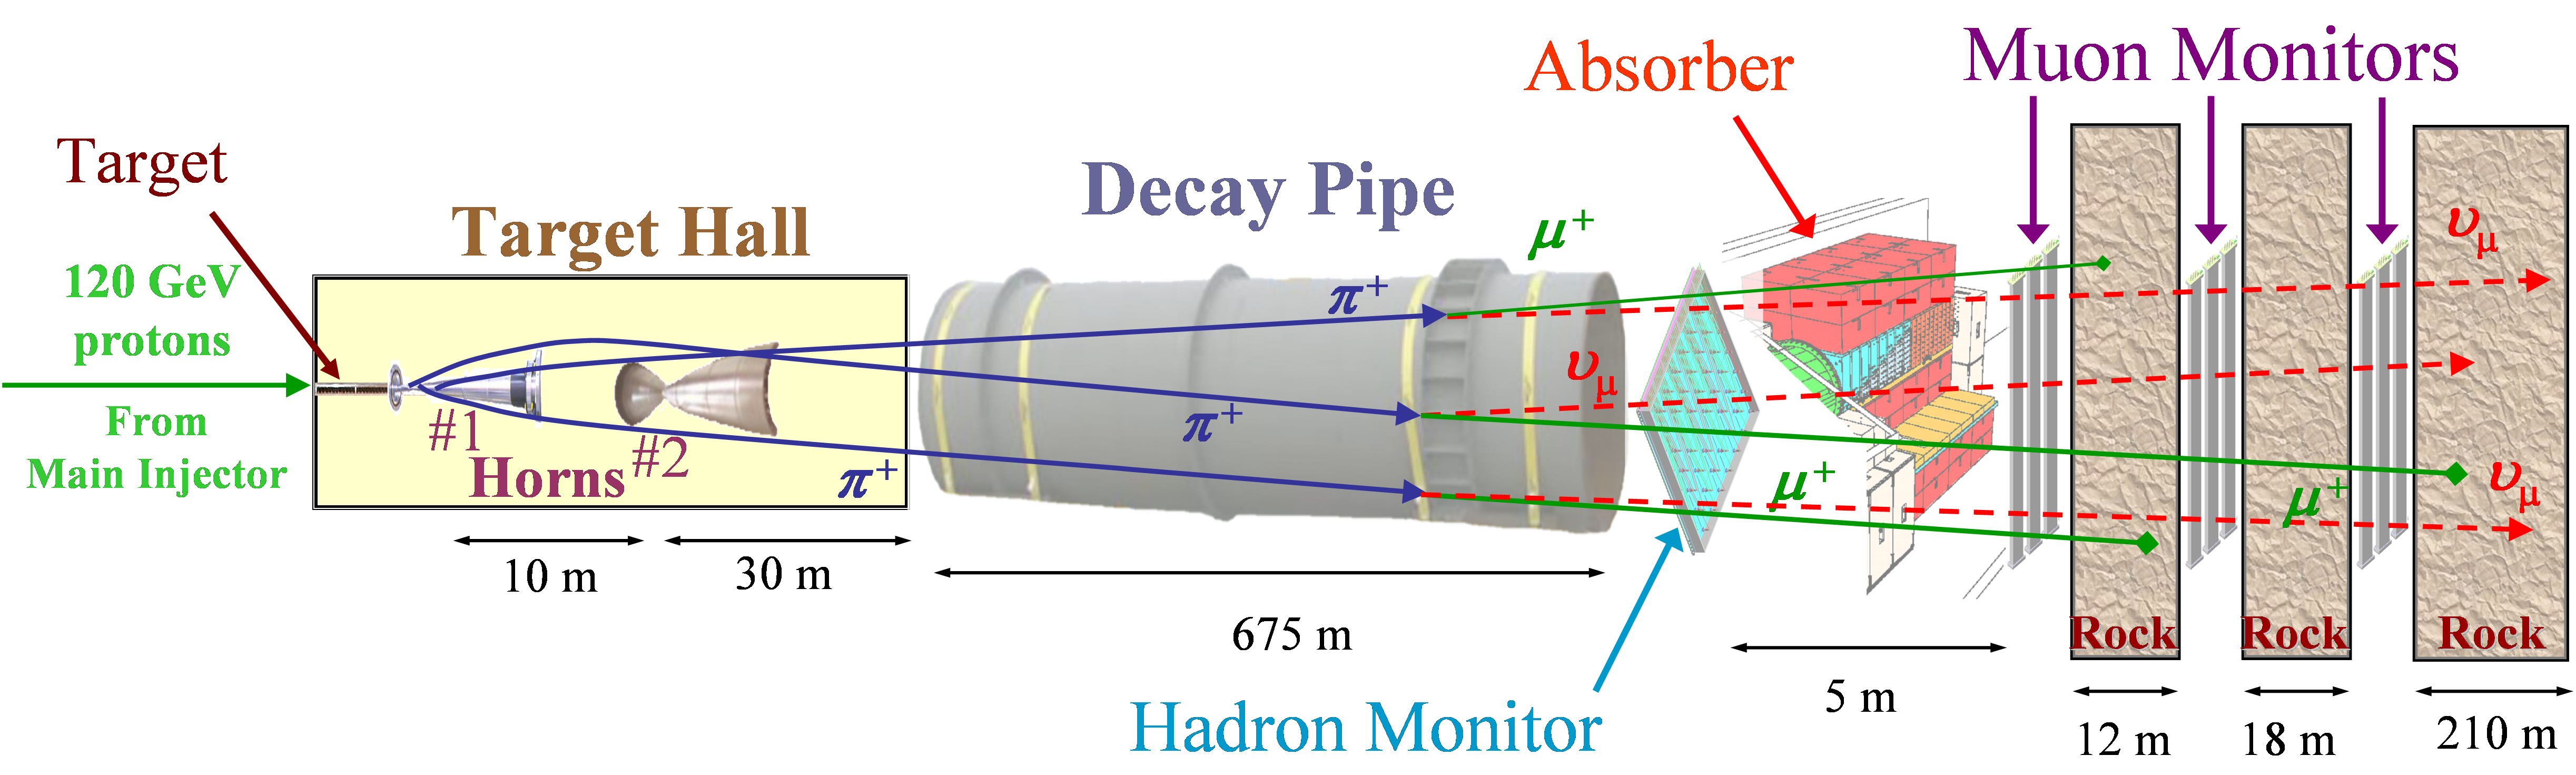
\includegraphics[width=1.0\textwidth]{figures/Beamline.png}
\centering
\caption{Schematics of neutrino production\cite{numi}.} \label{NuMI}
\end{figure}
Neutrinos for the NOvA experiments comes from decay of pions and kaons. To get a beam of 
the mesons Main Injector at Fermilab is used, which provides an intense beam of proton with 
energy 120 GeV. The structure of NuMI is illustrated on figure \p{NuMI}. It is designed to 
deliver $4.9 \times 10^{13}$ proton on target (POT) with the repetition rate of 1.3s, which 
corresponds to 700 kW of beam power. The proton beam is directed into a graphite target.  
Collisions between the proton beam and graphite target produces many types of hadrons and 
mesons, with pions and kaons among them. Magnetic focusing horns, which are supplied with 
current of 200kA, are used to focus and direct 
charged pions and kaons into a decay pipe. The decay pipe is long enough such that nearly all 
of the incoming pions and kaons decay before the end of the pipe. More than 99\% of all pions 
and 63\% of kaons decay into anti-muon/muon and muon/anti-muon neutrino, so the flux of 
particles at the end of the decay pipe consists of mostly muons and muon anti-neutrinos, or 
their antiparticles. By changing the electric current direction in the focusing horns one can 
switch between positively and negatively charged pions and kaons which enter the decay pipe. 
This gives an opportunity to make two types of neutrino beams - $\nu_\mu$'s and $\bar{\nu}_\mu$'s. 
Unfortunately, 5\% of charged kaons have electron neutrinos among their byproducts, and this 
is an irreducible background for an electron neutrino analysis. All the realitively long lived
charged particles such as muons and electrons do not reach Near Detector as they get absorbed 
in rock. A hadron monitor, absorber and muon monitor are placed at the end of decay pipe 
to better understand beam properties, but they do not play any role in the NOvA experiment.

\begin{wrapfigure}{r}{0.5\textwidth}
\vspace{-20pt}
  \begin{center}
    \includegraphics[width=0.48\textwidth]{figures/Neutrino_osc.png}
  \end{center}
\vspace{-30pt}
\end{wrapfigure}

After the neutrinos leave the decay pipe they begin their journey to the near and far detectors. 
There are a few reasons why the NO$\nu$A detectors are placed 14.6 mrad off-axis of the NuMI beam. 
As can be seen on the picture on the right, the first minimum of muon neutrino survival 
probability and first maximum of electron neutrino appearance probability are around 400 km/GeV 
but on-axis neutrino spectrum (black line on left picture \p{Spec}) does not allow to observe 
first maximum of $P(\nu_\mu \rightarrow \nu_e)$ for a baseline $~1000$ km. The solution is 
simple: pions and kaons decay isotropically in their rest frame but after Lorentz boost to 
laboratory frame flux and neutrino energy at the far detector (for small off-axis angles $\theta$) 
can be expressed in the following form
\be
F = \Big(\frac{2\gamma}{1+\gamma^2\theta^2}\Big)^2\frac{A}{4\pi d}
\ee
\be
E_\nu = \frac{0.43E_\pi}{1+\gamma^2\theta^2},
\ee
where $\gamma = \frac{E_\pi}{m_\pi}$, $A$ is the size of the detector front area and $d$ is 
the distance to the detector. For kaons numerical factor $0.43$ should be changed to $0.96$. 
Knowing the pion and kaon energy spectrum at the NuMI source, one can predict the neutrino energy 
spectrum at the far detector for different off-axis angles $\theta$. As shown on left side of 
\autoref{Spec}, the neutrino energy distribution gets narrower and shifts toward smaller energies. 
At 14.6 mrad the neutrino flux is still moderate and peaked near 2 GeV, which allows NOvA 
to study the region of maximal $P(\nu_\mu \rightarrow \nu_e)$ at 810 km. Moreover, the narrow 
peak decreases the chance that NC events from more energetic neutrinos could be misidentified 
as CC events in the energy region of interest. In general, the off-axis detector placement 
significantly improves the sensitivity of the probability measurement.
\begin{figure}
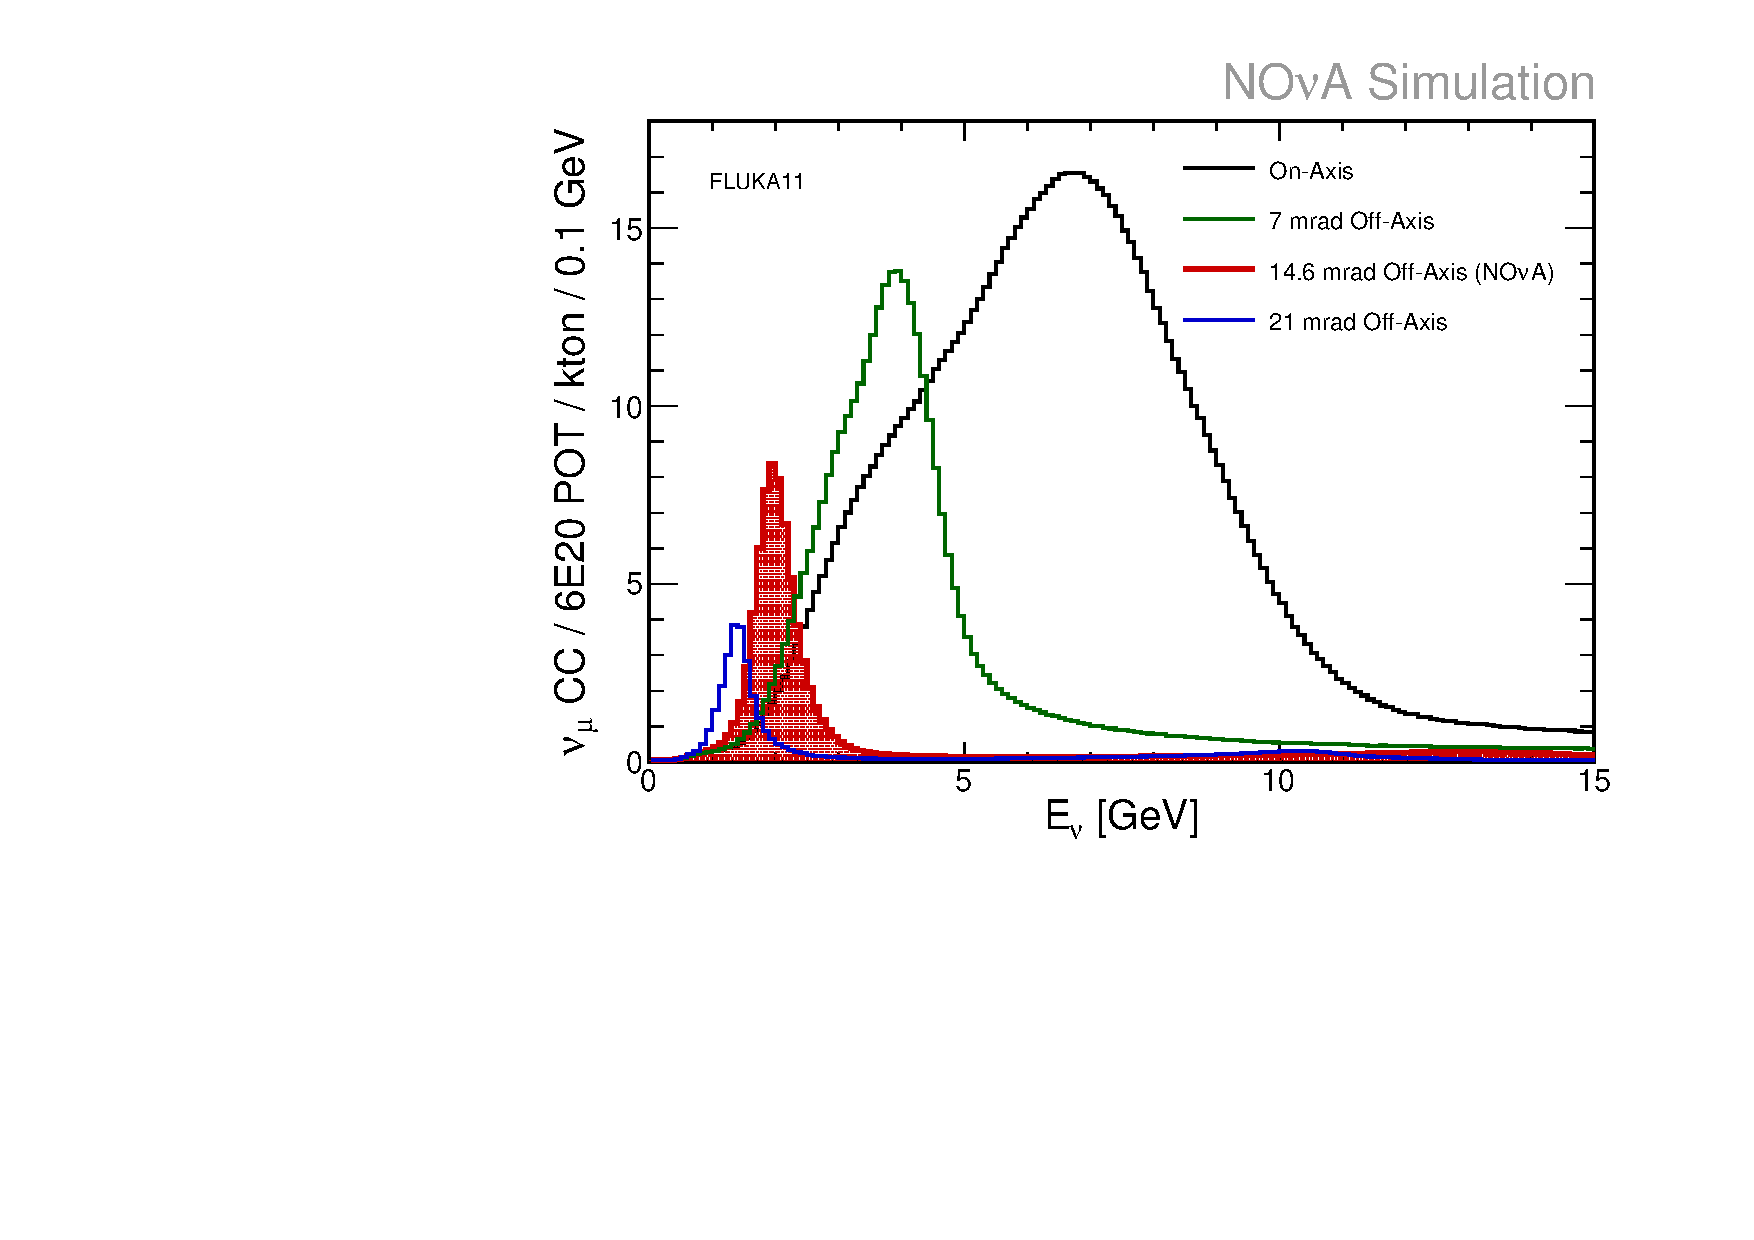
\includegraphics[width=0.9\textwidth]{figures/FD_NOvA_OffAxis_Spectra.pdf}\\%
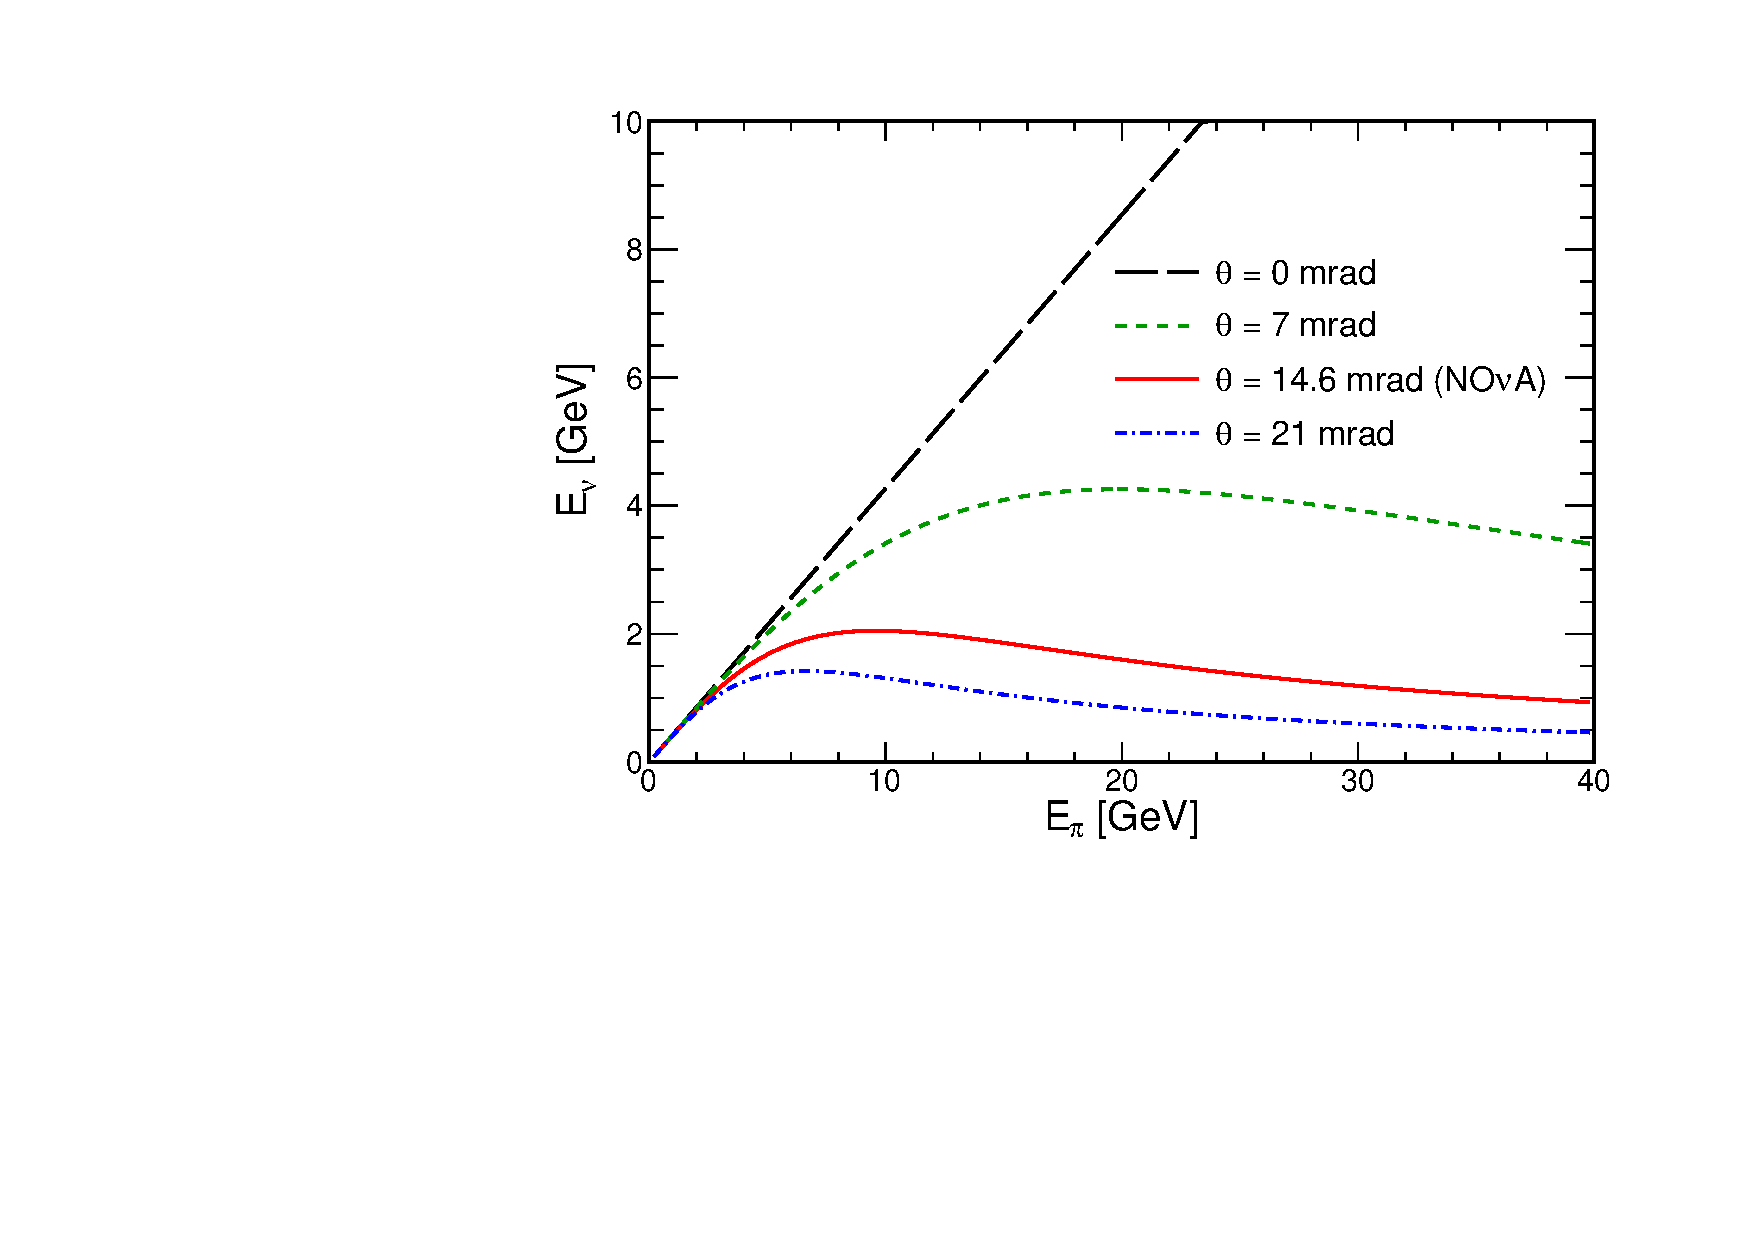
\includegraphics[width=0.9\textwidth]{figures/EnuVSEpi_NOvA.pdf}
\centering
\caption{(Left) Expected unoscillated neutrino spectrum at the Far Detector as a function of 
angle relative to NuMI beam. (Right)~Neutrino oscillation probabilities as a function of $\frac{L}{E}$, $
P(\nu_\mu \rightarrow \nu_\mu)$ - blue line, $P(\nu_\mu \rightarrow \nu_e)$ - black line and 
$P(\nu_\mu \rightarrow \nu_\tau)$ - red line.} \label{Spec}
\end{figure}
